\subsection{Динамическая теория рассеяния}
    При рассмотрении большинства физических процессов, задействованных
  в методах исследования структуры веществ с помощью рентгеновских лучей,
  используется математический аппарат волновой оптики.
  Плоская монохроматическая волна, распространяющая в вакууме, изображена на рисунке ~\ref{ris:plane_wave_vacuum},
  амплитуда плоских волн в вакууме $E_0$ не меняется с удалением от
  источника (в отличии от сферических или цилиндрических). В приближении плоской волны,
  плотность потока энергии, переносимой волной через единицу площади неизменна на любом расстоянии от источника.

  \begin{figure}[H]
    \centering
    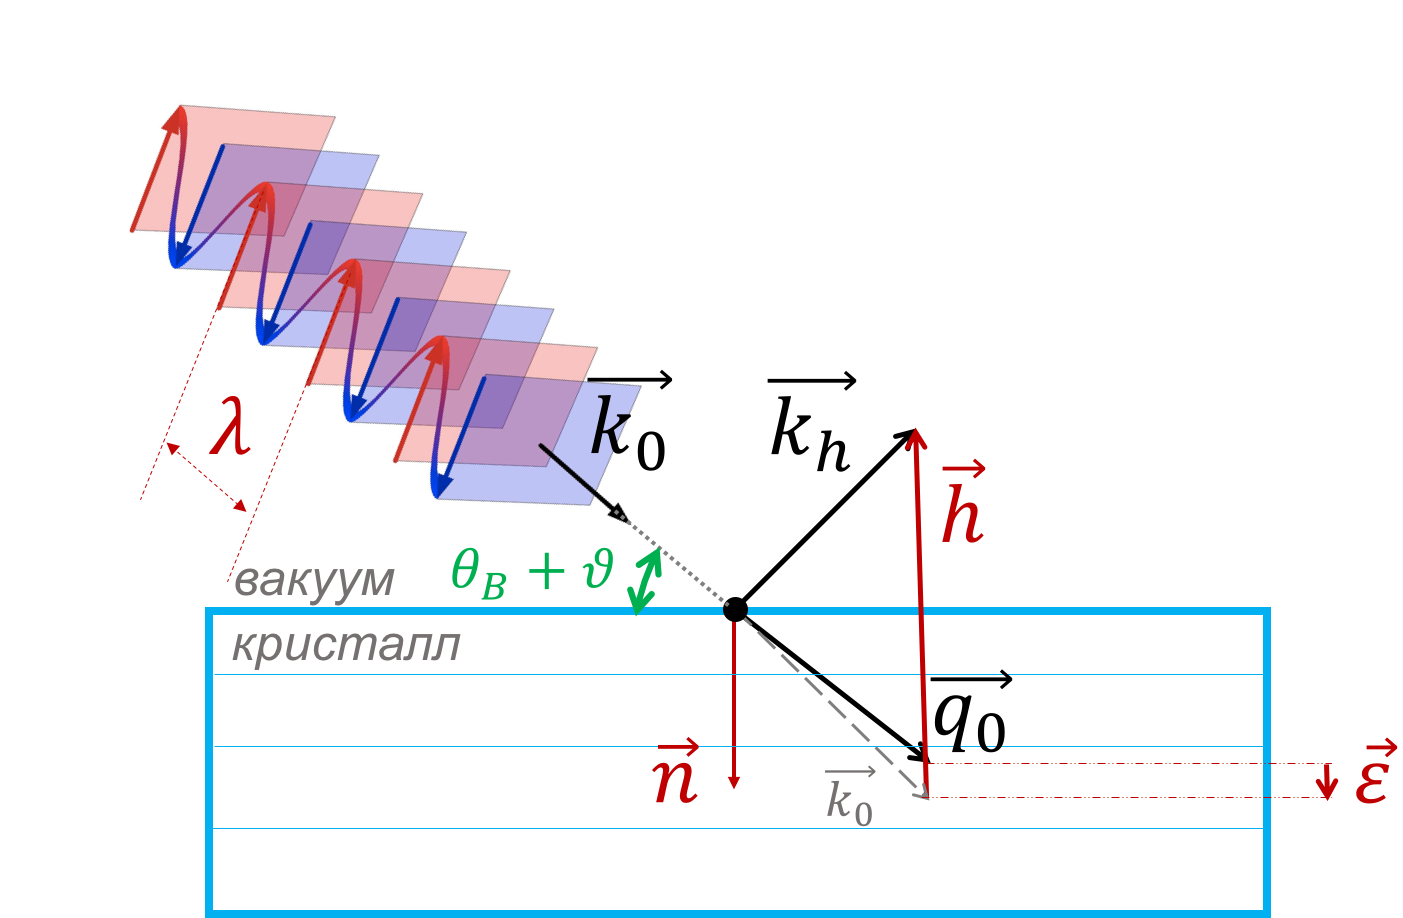
\includegraphics[width=0.8\textwidth]{images/plane_wave_vacuum.png}
    \caption{Схема к описанию динамической теории дифракции рентгеновского излучения с кристаллом.
      $\vec {k}$ - волновой вектор в вакууме; $\vec {q}$ - волновой вектор в среде;
     $0$ - коэффициент для обозначения падающей волны, а $h$ -  дифрагированной волны; $\vec{h}$ - вектор
     обратной решетки ($|h|=2\pi/d$); $\vec{n}$ - вектор нормали к поверхности, направленный внутрь объема;
     $\lambda$ - длина волны волнового вектора; $\vec{\varepsilon}$ - вектор аккомодации, характеризующий изменение
     волнового вектора в среде из-за преломления; $\vartheta$ - угол падения излучения на кристалл, для данного
     случая угол совпадает с углом Брегга $\vartheta = \theta_B$, т.к.  $\vec {k}_0 + \vec{h} = \vec {k}_h $}
    \label{ris:plane_wave_vacuum}
  \end{figure}

Рентгеновские лучи, как и видимы свет, распространяются параллельно и преломляются при
прохождении через границу раздела двух сред с разной оптической плотностью.
 Преломление рентгеновских лучей намного слабее, чем у видимого света, причем
 абсолютный показатель преломления рентгеновских лучей практически во всех средах
 практический одинаков и настолько близок к единице, что их преломление не удавалось обнаружить
 в течение тридцати лет после открытия рентгеновских лучей \cite{fetisov2007}, более того
 для рентгеновских лучей вакуум оказывается оптически наиболее плотной средой и луч
 при переходе в конденсированную среду увеличивает угол с нормалью к поверхности раздела сред ($n_{refr} \approx 1-10^{-5}$ ).
 Таким образом, волновой вектор, распространяющийся в вакууме отличается от своего продолжения в
 среде, но тангенциальная составляющая при переходе из одной среды в другу, в соответствии с теорией о циркуляции, сохраняется \cite{landau_8_1992}.

 \begin{equation}
   \vec{q}_0 = \vec{k}_0 + \varepsilon k_0 \cdot \vec{n}
  \end{equation}

Квадрат вектора,

\begin{equation}
   q_0^2 = k_0^2 + 2k_0^2 \varepsilon \cdot \gamma_0 + \cancelto{0}{k_0^4  \varepsilon^2}
   \label{eq:k_0_squred}
 \end{equation}

  где, $\gamma_0 = \cos(\vec{k}_0 \textasciicircum \vec{n})$ - косинус угла между вектором $\vec{k}_0$ и нормалью к поверхности кристалла,
  последним слагаемым можно пренебречь в силу его малости ($\sim 10^{-6}$).
  Волновой вектор дифрагированной волны, в соответствии с условием Брегга,

  $$\vec{k}_h = \vec{k}_0+\vec{h}$$

  \begin{equation}
     k_h^2 = \vec{k}_0^2+2k_0^2 \varepsilon \cdot \gamma_h
     \label{eq:k_h_squred}
   \end{equation}
   где, $\gamma_h = \cos(\vec{k}_0+ \vec{h} \textasciicircum \vec{n})$ - косинус угла между вектором $\vec{k}_h$ и нормалью к поверхности кристалла.

Для дальнейшего рассмотрения уравнения связывающего амплитуду падающей и дифрагированной волн в рамках
динамической теории рассеяния введем следующий параметр $\alpha$, характеризующий степень отклонения от условия Брегга.
\begin{equation}
   \alpha = \frac{k_0^2-k_h^2}{k_0^2}
   \label{eq:alpha}
\end{equation}


$$  \alpha = 1 - \frac{|\vec{k}_0|^2+2|\vec{k}_0||\vec{h}|\cos(\vec{k}_0 \textasciicircum \vec{h})+|\vec{h}|^2}{k_0^2}$$

учитывая, что $ |h| = 2|k_0| \sin(\theta_B) $, а $\vec{k}_0 \textasciicircum \vec{h} = 90-\theta_B+\vartheta$, получим:

\begin{equation}
   \alpha = -4\sin(\theta_B)(\sin(\theta_B+\vartheta)-\sin(\theta_B))
\end{equation}

  \subsubsection{Асимметричная схема дифракции}
В том случае если рентгеновское излучение отражается от атомных плоскостей не
 параллельных поверхности, в таком случае говорят об асимметрии отражения (рисунок ~\ref{ris:assymetric_brag}).

\begin{figure}[h]
  \centering
  \subfloat[$b >> 1$, $\varphi$ > 0]{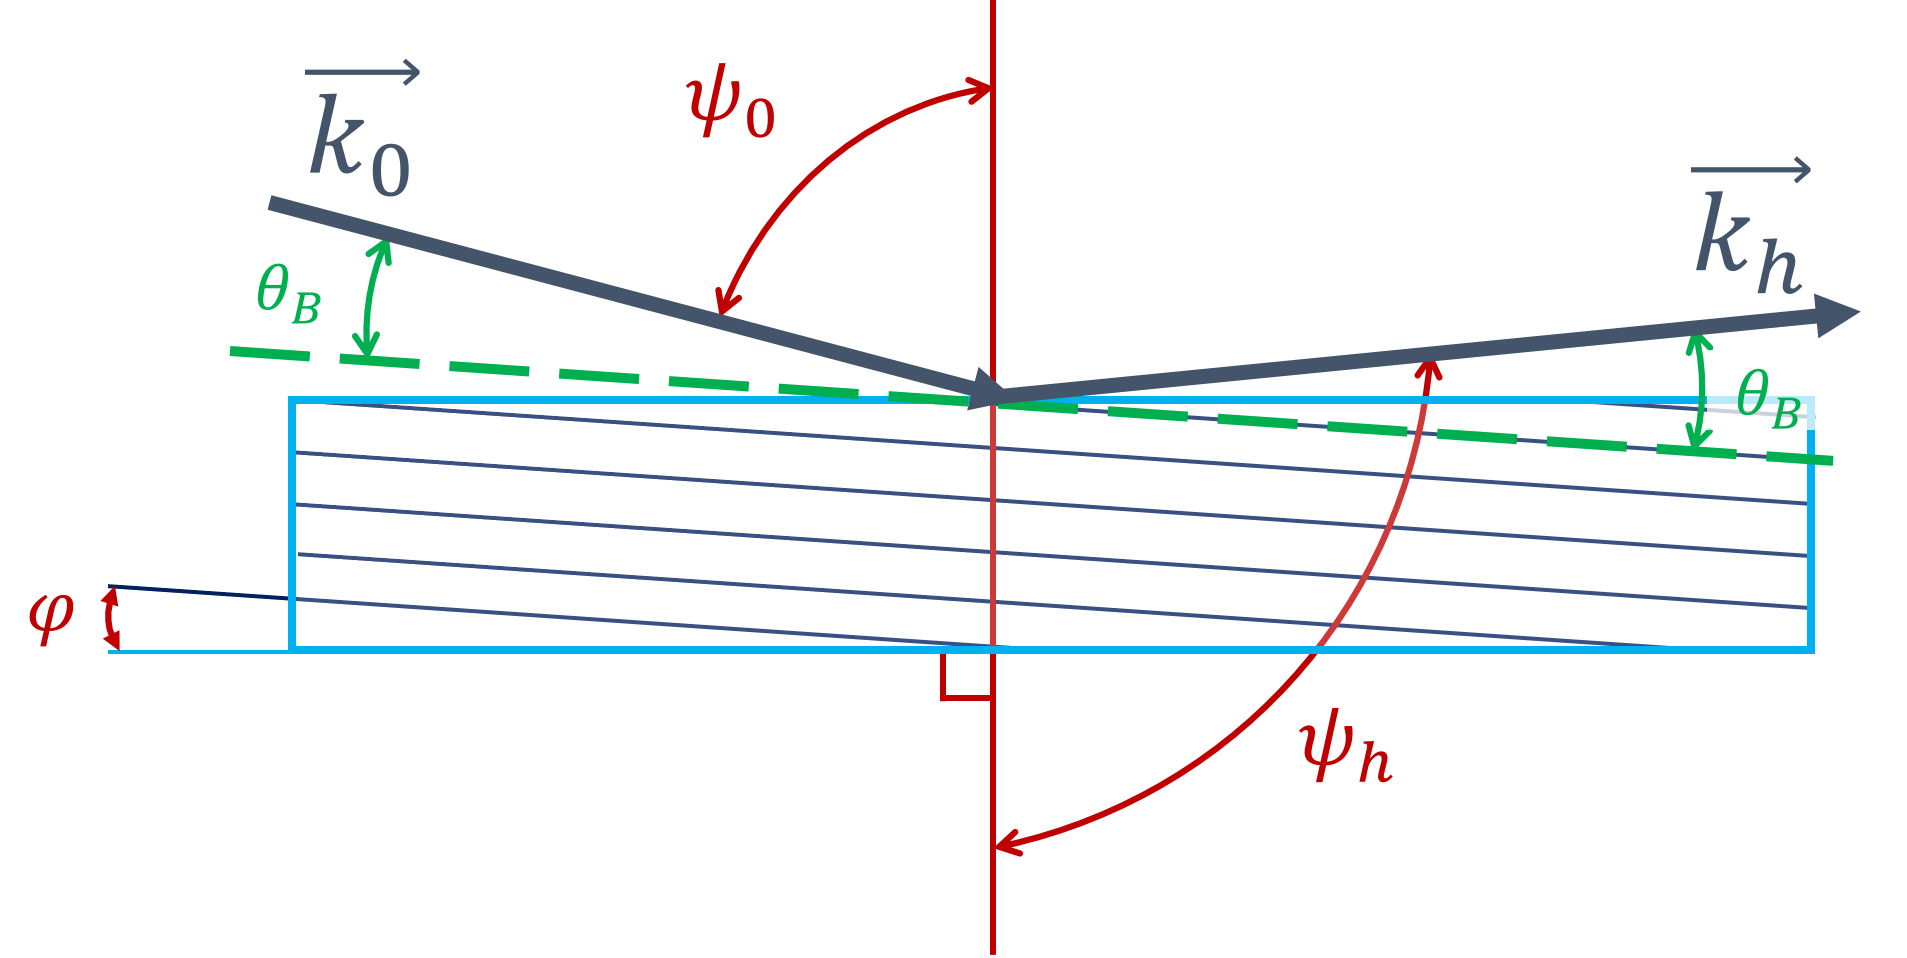
\includegraphics[width=0.45\textwidth]{images/assym2.png}\label{fig:f1}}
  \hfill
  \subfloat[$b << 1$, $\varphi$ < 0]{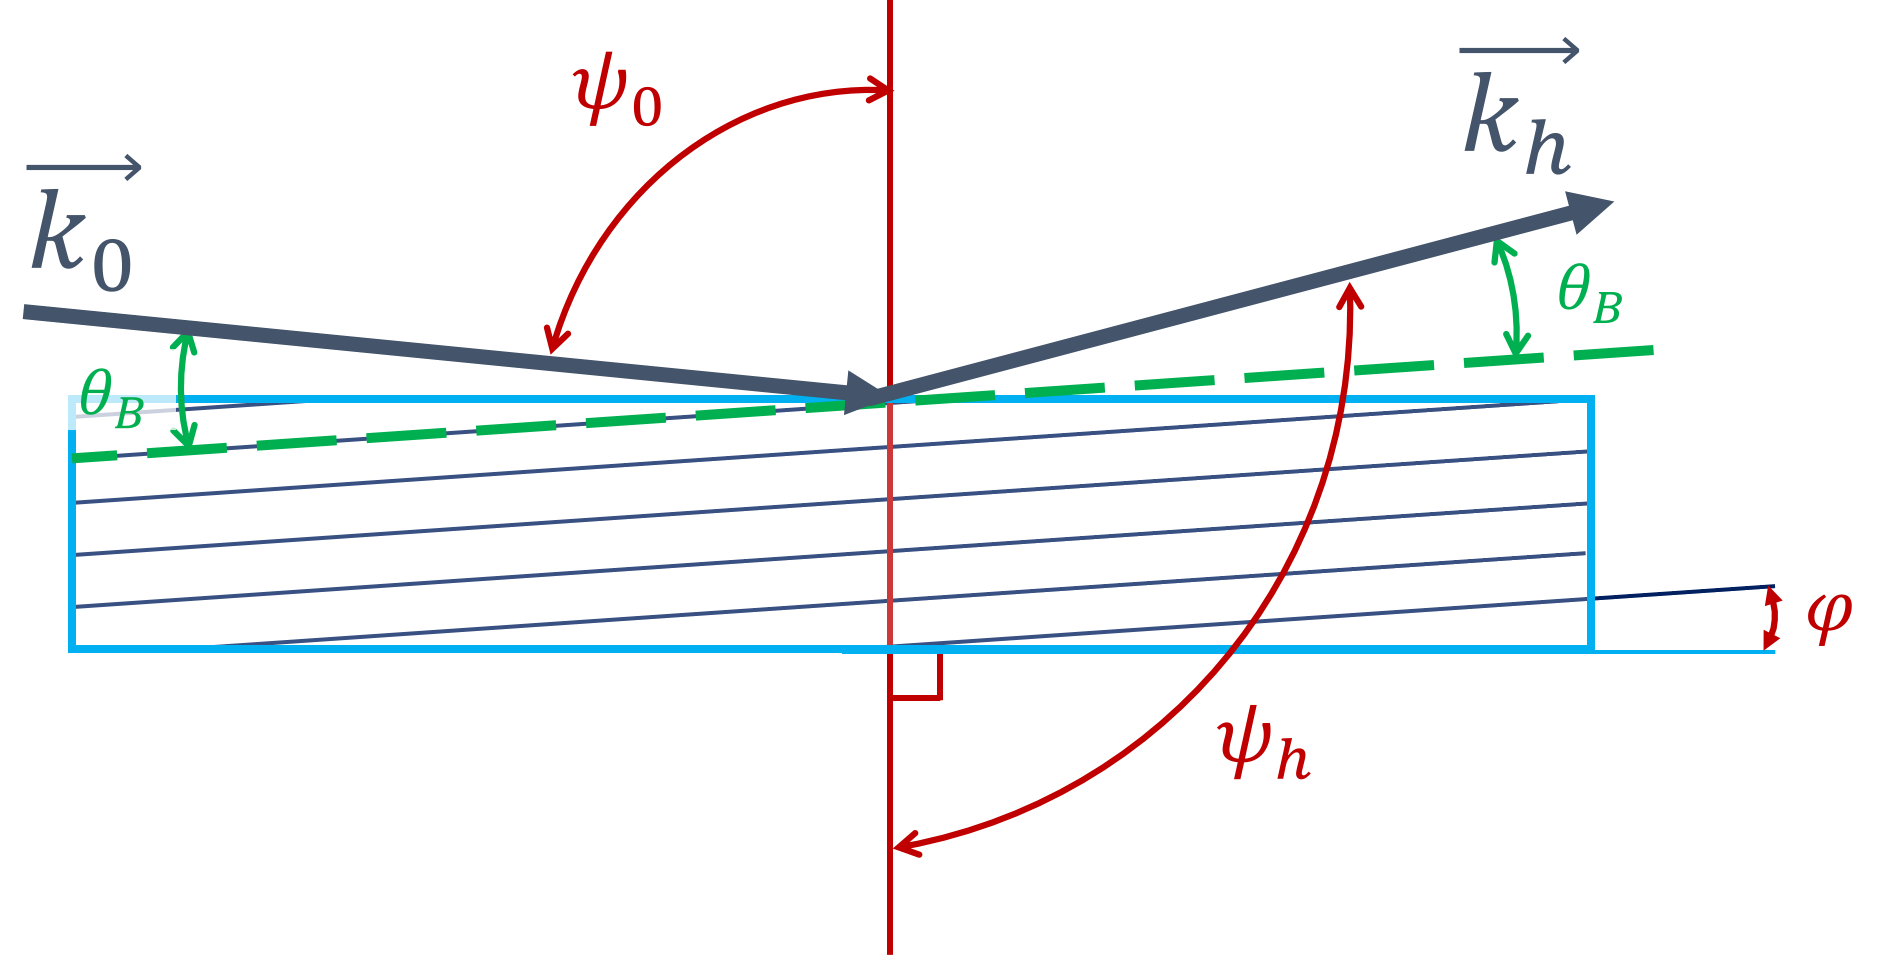
\includegraphics[width=0.45\textwidth]{images/assym1.png}\label{fig:f2}}
  \caption{Схема Брегговской дифракции для асимметричного отражения}
  \label{ris:assymetric_brag}
\end{figure}

Для того чтобы охарактеризовать степень асимметрии, введем коэффициент $b$:

\begin{equation}
  b = \frac {\gamma_0}{|\gamma_h|}
 \end{equation}
где, $\gamma_0 = cos \psi_0 = sin ( \varphi + \theta_B)$, $\gamma_h = cos \psi_h = sin ( \varphi - \theta_B)$,
$\varphi$ - угол между плоскостью отражения и поверхностью образца.


Весьма наглядной иллюстрацией являются собственные кривые отражения от Si(440) рассчитанные при
трех разных углах падения и соответсвенно имею разный коэффициент асимметрии. Угол
Брегга для такой плоскости отражения составляет $\theta_B = 21.68^o$, угол наклона поверхности
составляет $\varphi = 20^o 53^{'}$.

\begin{figure}[H]
\centering
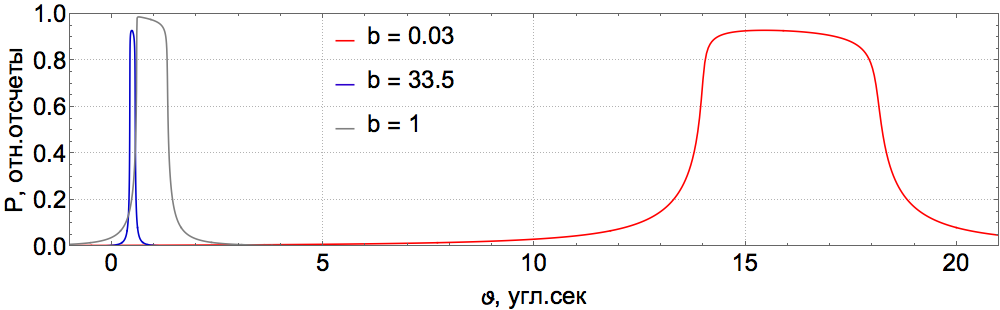
\includegraphics[width=0.99\textwidth]{images/rocking_curve_assym_3.png}
\caption{Кривые отражения 440 $MoK_{\alpha 1}$ от Si, полученные при разных углах падения(для разных b)}
\label{ris:rocking_curve_assym_3}
\end{figure}
Сдвиг центра кривой происходит из-за наличия преломления на величину 0.5 и 16.5 угловых секунд.

Варьируя угол между поверхностью кристалла и отражающей плоскостью (например, с помощью шлифовки),
можно существенно изменить ширину рентгеновского пучка (рисунок ~\ref{ris:assym_width_beam}).
\begin{figure}[H]
 \centering
 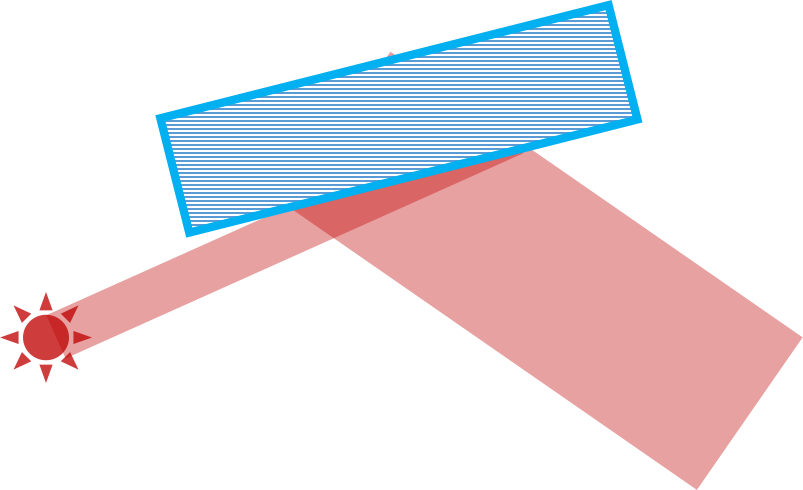
\includegraphics[width=0.4\textwidth]{images/assym_width_beam.png}
 \caption{Кристалл с асимметричным отражением по Бреггу}
 \label{ris:assym_width_beam}
\end{figure}



 % \input{maxwels_equation.tex}
 \subsubsection{Система уравнений Максвелла}

 Вне кристалла, падающая волна описывается в виде совокупности плоских волн с волновым вектором  $\vec{k_0}$.
 \begin{equation}
   \vec{E}_0(\vec{r},t) = E_0 e^{i(\vec{k}_0\vec{r}-\omega t)}
  \end{equation}

Падающая волна $vec{E}(\vec{r},t)_0$ порождает волновое поле внутри кристалла, которое характеризуется вектором
электромагнитной индукции $\vec{D}||\vec{E}$
\begin{equation}
  \vec{D}_0(\vec{r},t) = (1+\chi(\vec{r})) E_0 e^{i(\vec{k}_0\vec{r}-\omega t)} = A(r) e^{i(\vec{k}_0\vec{r}-\omega t)}
 \end{equation}

Амплитуда волны $A(\vec{r})$ - не зависит от времени, но зависит от координат, связано
это с тем что электроны колеблются под действие распространяющейся волны, и испускаемые ими
электромагнитные волны интерферируют между собой и с исходной волной. Устанавливается некоторое стабильное
электромагнитное поле с переодически изменяющейся в пространстве амплитудой. Периодичность эта должна быть
той же, что и периодичность решетки.

 В дальнейшем описании мы так же будем пренебрегать вектором магнитного поля и
 будем искать стабильное (не зависящее от времени) решение в виде совокупности плоских волн
